\documentclass[aspectratio=169]{beamer}
\usepackage[english]{babel}
\usepackage{xcolor}
\usepackage{transparent}
\usepackage[default,scale=1]{opensans}
\usepackage[T1]{fontenc}
\usepackage[utf8]{inputenc}
%\usepackage{algorithm} 
%\usepackage{algpseudocode}
%\usepackage{algorithmic}

\mode<presentation>
{
	\usefonttheme{structurebold}  % or try serif, structurebold, ...
%Uncomment the following to display navigation symbols
	\setbeamertemplate{navigation symbols}{}
	%Constructing the frame title
	\setbeamertemplate{frametitle}{% 
		\kern1em\hskip-15pt
		\usebeamercolor[fg]{section}% 
		\usebeamerfont{section}% 
		\insertsection
	}
	%Constructing the footline
	\setbeamertemplate{footline}{% 
		\kern1em\hskip3em% 
		
\includegraphics[width=0.3\textwidth]{ntnulogo_eng.png}
		\hfill% 
		\usebeamercolor[fg]{page number in head/foot}% 
		\usebeamerfont{page number in head/foot}% 
		\insertframenumber%
%Uncomment the following line to display the total number of pages in the footnote
		%\,/\,\inserttotalframenumber
		\hskip12pt%
		\kern1.5em\vskip2em% 
}
	%Defining fonts
	\setbeamerfont{title}{shape=\bfseries, size=\huge}
	\setbeamerfont{subtitle}{series=\mdseries,size=\Large}
	
	%Defining the colors. Here you can find more elements whose color can be modified:
	%http://www.cpt.univ-mrs.fr/~masson/latex/Beamer-appearance-cheat-sheet.pdf
	\definecolor{NTNUBlue}{HTML}{00509e}
	\definecolor{LightGrey}{HTML}{D3D3D3}
	\setbeamercolor{background canvas}{bg=NTNUBlue}
	\setbeamercolor{title}{fg=white}
	\setbeamercolor{subtitle}{fg=white}
	\setbeamercolor{date}{fg=LightGrey}
	\setbeamercolor{author}{fg=LightGrey}
	\setbeamercolor{frametitle}{fg=NTNUBlue}
	\setbeamercolor{itemize item}{fg=NTNUBlue}
	\setbeamercolor{enumerate item}{fg=NTNUBlue}
	\setbeamercolor{block title}{fg=NTNUBlue}
} 
	% Enforcing the final page
	\AtEndDocument{\begin{frame}[plain, noframenumbering]
		\begin{center}
			\vspace{4em}
			{\huge Thank your for your attention}\\
			\vspace{5em}
			
\includegraphics[width=0.7\textwidth]{ntnulogo_eng.png}
		\end{center}
	\end{frame}
	}

% ---------->	Write here the content of the front page <----------
	\title[Your Short Title]{Inferring learning rule parameters from neural spike data}
	\subtitle{Master thesis presentation, NTNU, 07.05.20\\ Astrid Langsrud\\ Supervisor: Benjamin Dunn\\ Co-Supervisor: Claudia Battistin
}
	\institute{
\includegraphics[width=0.7\textwidth]{ntnulogo_eng_neg.png}}
	%Remember to uncomment the 3 lines in the next section in order to dsplay the author
	\author{Name of the author}
	%Remember to uncomment the 3 lines in the next section in order to dsplay the date
	\date{\today}

\begin{document}
	
	%----------------------------------Constructing the front page----------------------------------
	\begin{frame}[plain, noframenumbering]
		\vfill
		\centering	
		\begin{beamercolorbox}[sep=8pt,center,colsep=-4bp,rounded=true,shadow=true]{institute}
			\usebeamerfont{institute}\insertinstitute
		\end{beamercolorbox}	
		\vskip2.5em\par
		{\usebeamercolor[fg]{titlegraphic}\inserttitlegraphic\par}	
		\begin{beamercolorbox}[sep=8pt,center,colsep=-4bp,rounded=true,shadow=true]{title}
			\usebeamerfont{title}\MakeUppercase{\inserttitle}\par%
			\ifx\insertsubtitle\@empty%
			\else%
			\vskip0.5em%
			{\usebeamerfont{subtitle}\usebeamercolor[fg]{subtitle}\insertsubtitle\par}%
			\fi%     
		\end{beamercolorbox}%
		
% ---------->	Uncomment the following to display author information <----------
		%	\begin{beamercolorbox}[sep=8pt,center,colsep=-4bp,rounded=true,shadow=true]{author}
		%		\usebeamerfont{author}\insertauthor
		%	\end{beamercolorbox}
		
% ---------->	Uncomment the following to display date <----------
		%	\begin{beamercolorbox}[sep=8pt,center,colsep=-4bp,rounded=true,shadow=true]{date}
		%		\usebeamerfont{date}\insertdate
		%	\end{beamercolorbox}\vskip0.5em

% ---------->	If you add author or date, reduce the following space <----------
		\vskip4em
		
	\end{frame}
	
	%Setting the background color to none
	\setbeamercolor{background canvas}{bg=}
	
% ---------->	Uncomment these lines for an automatically generated table of contents. <----------
	%\begin{frame}{Outline}
	%  \tableofcontents
	%\end{frame}
	
	%----------------------------------Example section: Introduction----------------------------------
	\section{Neuroscience motivation}
	
	\begin{frame}{Neuroscience motivation}
		
		
		\begin{itemize}
			\item Brain: network of connected nerve cells
			\item Connection strengths are dynamical
			\item Basic mechanism for learning and memories
            \item \textbf{Aim: Characterize the change of connection strengths with time}
            \item \textbf{Motivation: Could be relevant for studying memory related diseases, such as Alzheimers}
        
        \end{itemize}
            
        \begin{figure}[H]
        %\centering
        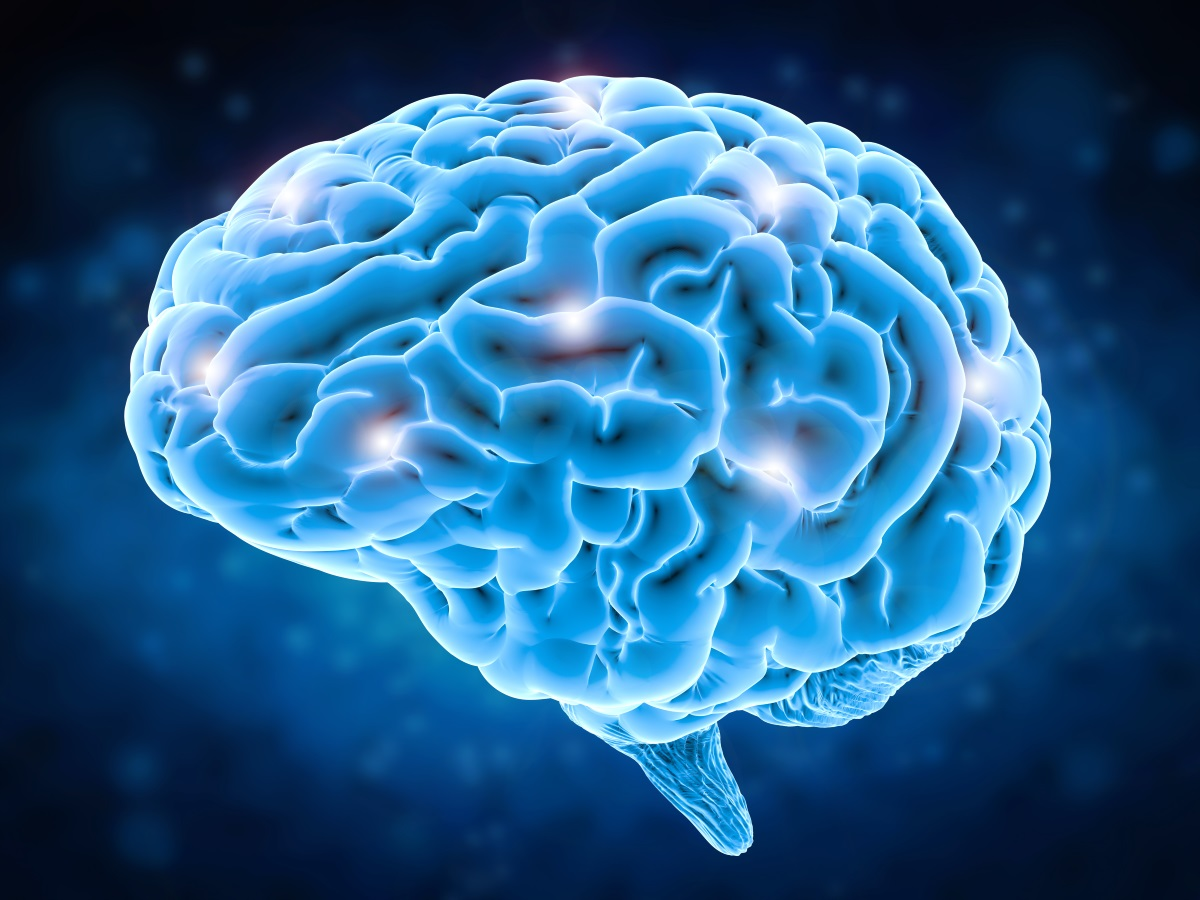
\includegraphics[scale=0.4]{Brain.jpg}
        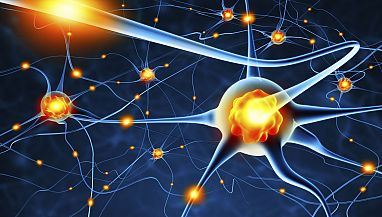
\includegraphics[scale=0.4]{Neurons.jpg}
        \vspace{-0.5cm}
        %\caption{}
        %\label{}
        \end{figure}

		
	\end{frame}	
	
	
	\section{Model framework}
	\begin{frame}{Model framework}
	
	    \begin{columns}[totalwidth=\textwidth]
        \begin{column}{0.7\textwidth}
            	\begin{itemize}
	            \item Neurons fire electrical impulses (spikes)
	            \item Data: Time points for spikes of \textit{neuron 1} and \textit{neuron 2}
	            \item The spike rate of \textit{neuron 2} at time $t$ is dependent on the connection strength at this time
	            \item Want to infer trajectory $\{W^t\}_{t=1}^T$
	            \end{itemize}
        \end{column}
        \begin{column}{0.3\textwidth}
            \begin{figure}[H]
            \centering
            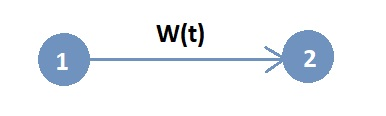
\includegraphics[scale=0.5]{Synapse.jpg}
            \vspace{-0.5cm}
            \end{figure}
        \end{column}
    \end{columns}

	\begin{columns}
	    \begin{column}{0.6 \textwidth}
	        \begin{figure}[]
            %\centering
            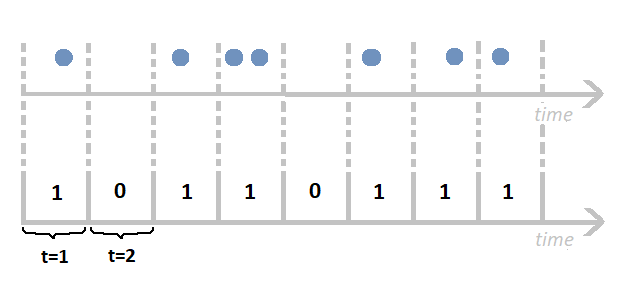
\includegraphics[scale=0.4, left]{Spike_train_illustration2.png}
            \vspace{-0.5cm}
            %\caption{}
            %\label{}
            \end{figure}
        \end{column}
        
        \begin{column}{0.4 \textwidth}
            \begin{equation}
                S_1^t \sim \text{Ber}(\mu_1) \hspace{0.5cm} S_2^t \sim \text{Ber}(\mu_2) \\
                \mu_1 = \text{logit}^{-1}(b_1)\\
                \mu_2 =\text{logit}^{-1}(W^t\cdot S_1^{t-1} + b_2) \nonumber
            \end{equation}
        \end{column}
    \end{columns}
	    
	\end{frame}
	
	\section{Learning rule}
	\begin{frame}{Learning rule}
	    %\begin{itemize}
	        %\item The connectivity strength, $\{W^t\}_{t=1}^T$ develops in time according to the neural activity, through a learning rule
	    %\end{itemize}
	    \begin{equation}
	        W^{t+1} = W^t + l(S^{1:t}, \theta) + \epsilon(\sigma) \nonumber
	   \end{equation}
	   \begin{equation}
	        \theta = \{A_+,A_-, \tau_+, \tau_- \}
	        \nonumber
	    \end{equation}
	    
	    \begin{itemize}
	        \item Activity dependent learning rule
	        \item Spike timing dependent plasticity (STDP) learning rule
	    \end{itemize}
	    
	    \begin{figure}[]
            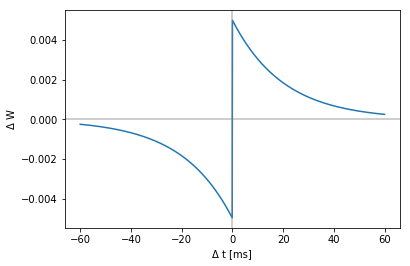
\includegraphics[scale=0.4]{LR_true.png}
            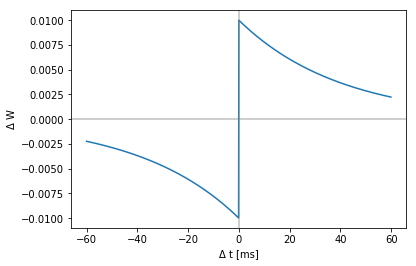
\includegraphics[scale=0.4]{LR_0.001_40}
            \vspace{-0.5cm}
            \end{figure}
	    %\begin{equation}
	            %l(S_1^{1:t}, S_2^{1:t}, \theta) = l_+(S_1^{1:t}, S_2^{1:t}, A_+, \tau_+) - l_-(S_1^{1:t}, S_2^{1:t}, A_-, \tau_-)\\
	            %l_+(S_1^{1:t}, S_2^{1:t}, A_+, \tau_+) = S_2^t \sum_{t'=1}^t S_1^{t'} A_+ e^{(t-t')/\tau_+}\\
	            %l_-(S_1^{1:t}, S_2^{1:t}, A_-, \tau_-) = S_1^t \sum_{t'=1}^t S_2^{t'} A_- e^{(t-t')/\tau_-} \nonumber
	    %\end{equation}
	
	\end{frame}
	
	\begin{frame}{Learning rule}
        \textbf{Goal: Infer learning rule parameters from spike data, and hence characterize $\mathbf{p(\theta |S^{1:T})}$}
	    
	    \begin{equation}
	        \theta = \{A_+,A_-,\tau_+, \tau_-  \} \nonumber
	    \end{equation}
	    
	    \begin{equation}
	        b_1, b_2, W^t, \sigma
	    \end{equation}
	\end{frame}
	
	\section{Particle Metropolis Hastings}
	
	\begin{frame}{Particle Metropolis Hastings}
	    \begin{itemize}
	        \item Bayesian approach, $p(\theta|S^{1:T}) \propto p(S^{1:T}|\theta)p(\theta) $
	        \item Can calculate approximation $\hat{p}(S^{1:T}|\theta)$ from $\hat{p}(W^{1:T}|S^{1:T}, \theta)$
	        \item Metropolis Hastings for inference on $\theta$ including particle filtering step to approximate $p(W^{1:T}|S^{1:T}, \theta)$
	    \end{itemize}
	\end{frame}
	
	\begin{frame}{Particle Metropolis Hastings}
	    \begin{figure}
	        \centering
	        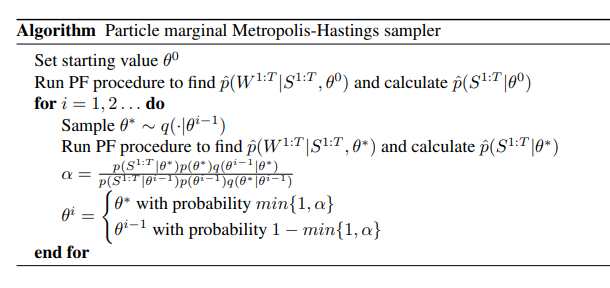
\includegraphics[scale=0.8]{PMCMC3.png}
	    \end{figure}

	    
	\end{frame}
	
	\section{Particle Filtering}
	

	
	\begin{frame}{Particle Filtering}
	
	\begin{columns}
	    \begin{column}{0.5 \textwidth}
        	    \begin{itemize}
        	        \item Approximate $p(W^{1:T}|S^{1:T}, \theta^*)$ with atomic distribution
        	    \end{itemize}
        	    
            \begin{equation}
                \hat{p}(W^{1:T}|S^{1:T}, \theta^*) = \sum_p \delta_{W^{1:T}_p} (W^{1:T}) \widetilde{v}^T_p
            \end{equation}
            
            \begin{itemize}
	           \item Sequential importance sampling
	        \end{itemize}
    
    \end{column}

	\begin{column}{0.5 \textwidth}
	\begin{figure}
	    \centering
	    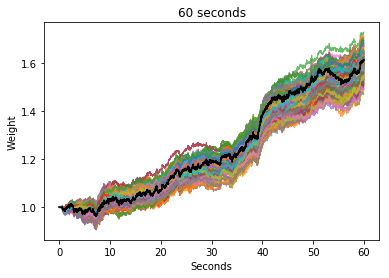
\includegraphics[scale = 0.5]{true_60.png}
	\end{figure}
	
	
	\end{column}
	
	\end{columns}
	    
	\end{frame}	
	
	\begin{frame}{Particle Filtering}
	    \begin{figure}
	        \centering
	        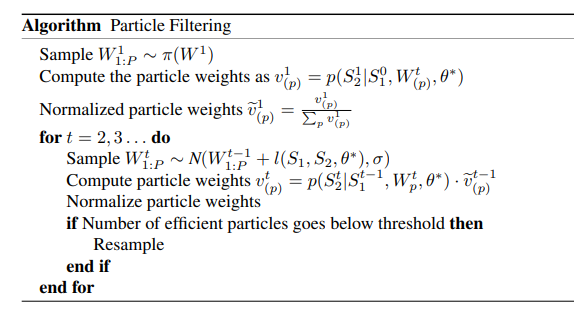
\includegraphics[scale = 0.8]{Particle_Filtering.png}
	    \end{figure}
	\end{frame}
	
	\begin{frame}{Particle Filtering}
	    \begin{figure}
	        \centering
	        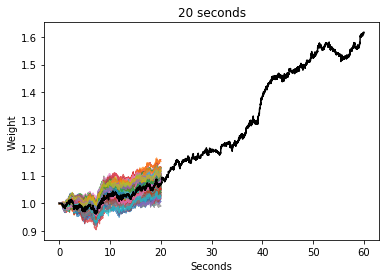
\includegraphics[scale=0.4]{true_20.png}
	        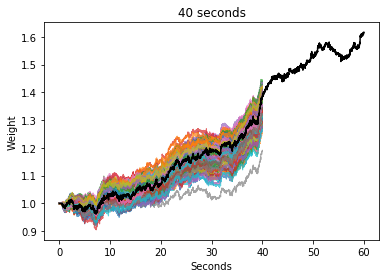
\includegraphics[scale=0.4]{true_40.png}\\
	        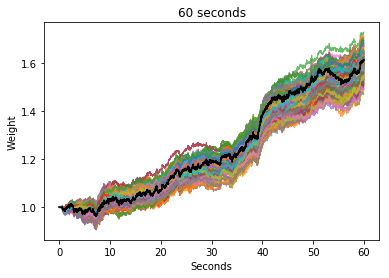
\includegraphics[scale=0.4]{true_60.png}
	    \end{figure}
	\end{frame}
	
	\section{Results: learning parameter A}
	
	\begin{frame}{Results: learning parameter A}
	
	    \begin{figure}
	        \centering
	        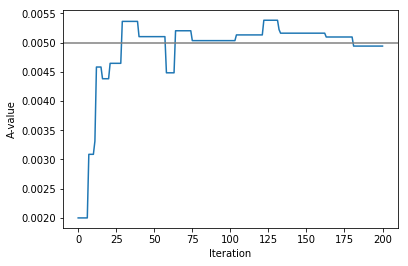
\includegraphics[scale=0.4]{240_0.0001.png}
	        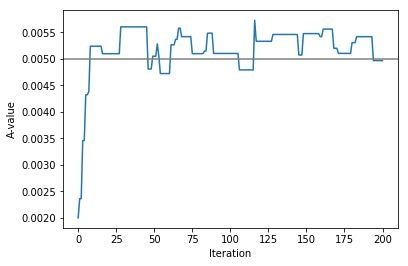
\includegraphics[scale=0.4]{240_0.0005.png}\\
	        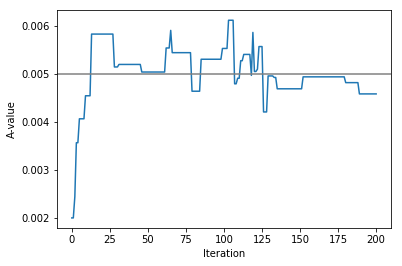
\includegraphics[scale=0.4]{240_0.001.png}
	        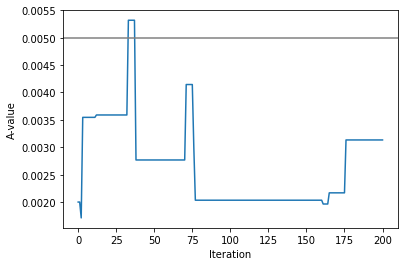
\includegraphics[scale=0.4]{240_0.005.png}
	    \end{figure}
	    
	\end{frame}
	
	\section{Further work}
	
	\begin{frame}{Further work}
	    
	\end{frame}
	
	\section{References}
	
	\begin{frame}{References}
	    
	\end{frame}
\end{document}
